\documentclass[a4paper]{article}

\usepackage{amsmath, amssymb, amsthm,stackengine}
\usepackage{tikz}
\usepackage{mathtools}
\usepackage{multicol}
\usepackage[top=0.5cm,left=0.5cm,right=0.5cm,bottom=0.5cm]{geometry}
\usepackage{amsfonts}
\usepackage{etoolbox}
\usepackage{cancel}
\usepackage{yhmath}
\usepackage{hyperref}
\usepackage{graphicx}
\usepackage{caption}
\usepackage[overload]{empheq} % For braced-style systems of equations.

\usepackage{bm}
%\usepackage{enumerate}
\usepackage{enumitem}
\usepackage{centernot}
\usepackage{tikz}
\newcommand{\circled}[1]{%
  \tikz[baseline=(char.base)]\node[shape=circle,draw,inner sep=2pt] (char) {#1};%
}

\newtheoremstyle{break}
  {\partopsep}{\topsep}%  
  {\itshape}{}
  {\bfseries}{}%
  {\newline}{}%
  \theoremstyle{break}
\newtheorem*{theorem}{Theorem}

\usepackage[framemethod=TikZ]{mdframed}

\mdfdefinestyle{theoremstyle}{
    linecolor=red,
    linewidth=1pt,
    roundcorner=5pt,
    innertopmargin=2pt,
    innerbottommargin=2pt,
    innerrightmargin=4pt,
    innerleftmargin=4pt,
    backgroundcolor=red!10,
    nobreak=true,
    leftmargin=0pt,
    rightmargin=0pt,
    skipabove=3pt
}

\surroundwithmdframed[style=theoremstyle]{theorem}

%\usepackage[mathabx]{mathabx}

% Declare necessary fonts from mathabx
\DeclareFontFamily{U}{matha}{\hyphenchar\font45}
\DeclareFontShape{U}{matha}{m}{n}{
  <-6> matha5 <6-7> matha6 <7-8> matha7
  <8-9> matha8 <9-10> matha9
  <10-12> matha10 <12-> matha12
}{}
\DeclareSymbolFont{matha}{U}{matha}{m}{n}

% Declare necessary fonts from mathabx
\DeclareFontFamily{U}{mathb}{\hyphenchar\font45}
\DeclareFontShape{U}{mathb}{m}{n}{
  <-6> mathb5 <6-7> mathb6 <7-8> mathb7
  <8-9> mathb8 <9-10> mathb9
  <10-12> mathb10 <12-> mathb12
}{}
\DeclareSymbolFont{mathb}{U}{mathb}{m}{n}

\DeclareMathSymbol{\coloneq}       {3}{mathb}{"15}
\DeclareMathSymbol{\eqcolon}       {3}{mathb}{"16}
\DeclareMathSymbol{\subsetneqq}    {3}{matha}{"90}
\DeclareMathSymbol{\nLeftarrow}    {3}{matha}{"F6}
\DeclareMathAccent{\abxring}       {0}{mathb}{"38}

\newcommand{\impliesnotimplied}{%
  \mathrel{%
    \vcenter{\offinterlineskip
      \ialign{##\cr$\nLeftarrow$\cr\noalign{\kern+1pt}$\Rightarrow$\cr}%
    }%
  }%
}

\newenvironment{Figure}
  {\par\medskip\noindent\minipage{\linewidth}}
  {\endminipage\par\medskip}

\definecolor{forestgreen(web)}{rgb}{0.13, 0.55, 0.13}
\definecolor{lavender(floral)}{rgb}{0.71, 0.49, 0.86}

\usepackage{nicefrac, xfrac}
%\usepackage{mathtools}
\newcommand{\abs}[1]{\left\lvert #1 \right\rvert}
\newcommand{\norm}[1]{\left\lVert #1 \right\rVert}
\newcommand{\sca}[1]{\left\langle #1 \right\rangle}

%\usepackage{xcolor}
\usepackage{titlesec}

%\usepackage{wasysym}
%\smiley{}

\usepackage{tikzsymbols}


% Bold
\renewcommand{\AA}{\mathbb A}
\newcommand{\BB}{\mathbb{B}}
\newcommand{\CC}{\mathbb{C}}
\newcommand{\DD}{\mathbb{D}}
\newcommand{\EE}{\mathbb{E}}
\newcommand{\FF}{\mathbb{F}}
\newcommand{\GG}{\mathbb{G}}
\newcommand{\HH}{\mathbb{H}}
\newcommand{\II}{\mathbb{I}}
\newcommand{\JJ}{\mathbb{J}}
\newcommand{\KK}{\mathbb{K}}
\newcommand{\LL}{\mathbb{L}}
\newcommand{\MM}{\mathbb{M}}
\newcommand{\NN}{\mathbb{N}}
\newcommand{\OO}{\mathbb{O}}
\newcommand{\PP}{\mathbb{P}}
\newcommand{\QQ}{\mathbb{Q}}
\newcommand{\RR}{\mathbb{R}}
\renewcommand{\SS}{\mathbb S}
\newcommand{\TT}{\mathbb{T}}
\newcommand{\UU}{\mathbb{U}}
\newcommand{\VV}{\mathbb{V}}
\newcommand{\WW}{\mathbb{W}}
\newcommand{\XX}{\mathbb{X}}
\newcommand{\YY}{\mathbb{Y}}
\newcommand{\ZZ}{\mathbb{Z}}

% Calligraphic
\newcommand{\Ac}{\mathcal{A}}
\newcommand{\Bc}{\mathcal{B}}
\newcommand{\Cc}{\mathcal{C}}
\newcommand{\Dc}{\mathcal{D}}
\newcommand{\Ec}{\mathcal{E}}
\newcommand{\Fc}{\mathcal{F}}
\newcommand{\Gc}{\mathcal{G}}
\newcommand{\Hc}{\mathcal{H}}
\newcommand{\Ic}{\mathcal{I}}
\newcommand{\Jc}{\mathcal{J}}
\newcommand{\Kc}{\mathcal{K}}
\newcommand{\Lc}{\mathcal{L}}
\newcommand{\Mc}{\mathcal{M}}
\newcommand{\Nc}{\mathcal{N}}
\newcommand{\Oc}{\mathcal{O}}
\newcommand{\Pc}{\mathcal{P}}
\newcommand{\Qc}{\mathcal{Q}}
\newcommand{\Rc}{\mathcal{R}}
\newcommand{\Sc}{\mathcal{S}}
\newcommand{\Tc}{\mathcal{T}}
\newcommand{\Uc}{\mathcal{U}}
\newcommand{\Vc}{\mathcal{V}}
\newcommand{\Wc}{\mathcal{W}}
\newcommand{\Xc}{\mathcal{X}}
\newcommand{\Yc}{\mathcal{Y}}
\newcommand{\Zc}{\mathcal{Z}}

% Bold Big Vector
\newcommand{\Av}{\mathbf{A}}
\newcommand{\Bv}{\mathbf{B}}
\newcommand{\Cv}{\mathbf{C}}
\newcommand{\Dv}{\mathbf{D}}
\newcommand{\Ev}{\mathbf{E}}
\newcommand{\Fv}{\mathbf{F}}
\newcommand{\Gv}{\mathbf{G}}
\newcommand{\Hv}{\mathbf{H}}
\newcommand{\Iv}{\mathbf{I}}
\newcommand{\Jv}{\mathbf{J}}
\newcommand{\Kv}{\mathbf{K}}
\newcommand{\Lv}{\mathbf{L}}
\newcommand{\Mv}{\mathbf{M}}
\newcommand{\Nv}{\mathbf{N}}
\newcommand{\Ov}{\mathbf{O}}
\newcommand{\Pv}{\mathbf{P}}
\newcommand{\Qv}{\mathbf{Q}}
\newcommand{\Rv}{\mathbf{R}}
\newcommand{\Sv}{\mathbf{S}}
\newcommand{\Tv}{\mathbf{T}}
\newcommand{\Uv}{\mathbf{U}}
\newcommand{\Vv}{\mathbf{V}}
\newcommand{\Wv}{\mathbf{W}}
\newcommand{\Xv}{\mathbf{X}}
\newcommand{\Yv}{\mathbf{Y}}
\newcommand{\Zv}{\mathbf{Z}}

% Bold Little Vector
\newcommand{\av}{\mathbf{a}}
\newcommand{\bv}{\mathbf{b}}
\newcommand{\cv}{\mathbf{c}}
\newcommand{\dv}{\mathbf{d}}
\newcommand{\ev}{\mathbf{e}}
\newcommand{\fv}{\mathbf{f}}
\newcommand{\gv}{\mathbf{g}}
\newcommand{\hv}{\mathbf{h}}
\newcommand{\iv}{\mathbf{i}}
\newcommand{\jv}{\mathbf{j}}
\newcommand{\kv}{\mathbf{k}}
\newcommand{\lv}{\mathbf{l}}
\newcommand{\mv}{\mathbf{m}}
\newcommand{\nv}{\mathbf{n}}
\newcommand{\ov}{\mathbf{o}}
\newcommand{\pv}{\mathbf{p}}
\newcommand{\qv}{\mathbf{q}}
\newcommand{\rv}{\mathbf{r}}
\newcommand{\sv}{\mathbf{s}}
\newcommand{\tv}{\mathbf{t}}
\newcommand{\uv}{\mathbf{u}}
\newcommand{\vv}{\mathbf{v}}
\newcommand{\wv}{\mathbf{w}}
\newcommand{\xv}{\mathbf{x}}
\newcommand{\yv}{\mathbf{y}}
\newcommand{\zv}{\mathbf{z}}

\renewcommand{\hat}{\widehat}

% differenziale
\newcommand{\dspace}{\ } % \, aggiunge un piccolo spazio
\newcommand{\de}{\mathrm{d}}
\newcommand{\dx}{\dspace \de x}
\newcommand{\dy}{\dspace \de y}
\newcommand{\dt}{\dspace \de t}
\newcommand{\dS}{\dspace \de S}
\newcommand{\ds}{\dspace \de s}
\newcommand{\dz}{\dspace \de z}
\newcommand{\dw}{\dspace \de w}
\newcommand{\du}{\dspace \de u}
\newcommand{\dvv}{\dspace \de v}
\newcommand{\db}{\dspace \de b}
\newcommand{\dteta}{\dspace \de \vartheta}
\newcommand{\dxi}{\dspace \de \xi}
\newcommand{\dxy}{\dspace \de x \de y}
\newcommand{\duv}{\dspace \de u \de v}
\newcommand{\dst}{\dspace \de s \de t}
\newcommand{\dP}{\dspace \de P}
\newcommand{\dPP}{\dspace \de \PP}
\newcommand{\dsig}{\dspace \de \sigma}
\newcommand{\dth}{\dspace \de \theta}
\newcommand{\deta}{\dspace \de \eta}
\newcommand{\dph}{\dspace \de \varphi}
\newcommand{\dxv}{\dspace \de \mathbf{x}}
\newcommand{\dSx}{\dspace \de \text{S}(x)}

\newcommand{\Bot}{\perp \!\!\! \perp} % indipendenza
\usepackage{dsfont} % per funzione indicatrice
\newcommand{\Ind}{\mathds{1}} % funzione indicatrice

\DeclareMathOperator{\Det}{det} % determinante
\DeclareMathOperator{\Img}{Im}
\DeclareMathOperator{\Ker}{Ker}
\DeclareMathOperator{\ArgMin}{ArgMin}
\DeclareMathOperator*{\esssup}{ess\,sup}
\DeclareMathOperator{\Div}{div}
\newcommand{\nabladot}{\nabla\!\!\cdot\!}
\DeclareMathOperator{\Lip}{Lip}

\renewcommand{\theta}{\vartheta}

%\DeclareMathOperator{\ker}{ker}
 
 % Turn off header and footer
\pagestyle{empty}

% Redefine section commands to use less space
\makeatletter

\renewcommand{\section}{\@startsection{section}{1}{0mm}%
                                {-0.1ex plus -.5ex minus -.2ex}%
                                {1.5ex plus .2ex}%x
                                {\center\normalfont\large\bfseries\color{red}}}

\renewcommand{\subsection}{\@startsection{subsection}{2}{0mm}%
                                {-0.1ex plus 0ex minus 0ex}%
                                {1.5ex plus 0ex}%
                                {\normalfont\scriptsize\color{red}}}

\makeatother

\titlespacing\section{0pt}{0pt plus 0pt minus 0pt}{0pt plus 0pt minus 0pt}

% Don't print section numbers
\setcounter{secnumdepth}{0}

\setlength{\parindent}{0pt}
\setlength{\parskip}{0pt plus 0ex}

% -----------------------------------------------------------------------

\begin{document}

\begin{equation*}
\boxed{
\int_\Omega \text{div}\,\fv\ g=\int_{\partial\Omega}\fv\cdot\nv\ g-\int_\Omega \fv\cdot\nabla g} \qquad \qquad
\boxed{
\int_\Omega \Delta u\ v=\int_{\partial\Omega}\frac{\partial u}{\partial n}\ v-\int_\Omega \nabla u\cdot\nabla v}
\end{equation*}

\bigskip

\raggedright
\footnotesize
\begin{multicols*}{2}

% multicol parameters
\setlength{\columnseprule}{1pt}
\def\columnseprulecolor{\color{red}}
\setlength{\premulticols}{1pt}
\setlength{\postmulticols}{1pt}
\setlength{\multicolsep}{1pt}
\setlength{\columnsep}{2pt}

%!TEX root = ../main.tex

% =================================================

\section{Diffusion / Elliptic Problems}

% =================================================

\textbf{BVP.} The general form of a Boundary Value Problem is
\begin{equation}
\label{eqn:general}
\begin{cases}
\Lc u = f & \text{in }\Omega \\
+\text{ bcs} & \text{on }\partial\Omega 
\end{cases}
\end{equation}
where
\begin{itemize}
\item $\Omega$: open bdd domain in $\RR^d$, with $d=2,\ 3$
\item $\partial\Omega$: \emph{reasonably} smooth boundary of $\Omega$
\item $f$: given datum
\item bcs: boundary conditions to be prescribed according to $\Lc$
\item $\Lc$: 2nd order differential operator which defines the PDE $\Lc u = f$ 
\end{itemize}

Examples:
\begin{itemize}
\item diffusion / Poisson equation
\begin{equation*}
\Lc u = -\Div\left( \mu_0 \nabla u \right)=-\mu_0 \Delta u
\end{equation*}
where $\mu_0>0$ is the diffusion coefficient
\item advection diffusion reaction (ADR) equation
\begin{align*}
\Lc u &= -\Div( \mu \nabla u )+\bv\cdot\nabla u+\sigma u &&\text{non-conservative} \\
\Lc u &= -\Div( \mu \nabla u )+\Div (\bv u)+\sigma u &&\text{conservative}
\end{align*}
where 
\begin{itemize}
\item $\mu\in L^\infty(\Omega)$, $\mu(\xv)\geq \mu_0>0$ (uniformly bdd from below)
\item $\bv \in \big[ L^\infty(\Omega) \big]^d$ is the advection / transport term
\item $\sigma \in L^\infty(\Omega)$, $\sigma(\xv)\geq 0$ is the reaction term
\item $f\in L^2(\Omega)$ (but it could be less regular)
\end{itemize}
\end{itemize}

If we consider mixed bcs, we have the following elliptic problem:
\begin{equation}
\label{eqn:ADRproblem}
\left\{
\begin{array}{lll}
\text{-}\Div( \mu \nabla u )+\bv\cdot\nabla u+\sigma u=f &\text{in }\Omega & \text{(ADR eq)} \\
u=0 &\text{on }\Gamma_D & \text{(Dirichlet/essential bc)} \\
\mu \nabla u \cdot \nv = g & \text{on }\Gamma_N & \text{(Neumann/natural bc)}
\end{array}
\right.
\end{equation}

where 

% Save the current parameters
\newlength{\oldcolumnseprule}

\setlength{\oldcolumnseprule}{\columnseprule}

% Set new parameters for the new multicol environment
\setlength{\columnseprule}{0pt} % No separator rule

\begin{multicols*}{2}
% Your content here
\begin{itemize}
\item $g\in L^2\!\left(\Gamma_N\right)$
\item $\partial\Omega=\Gamma_D \cup \Gamma_N$
\item $\abxring{\Gamma}_D\cap\abxring{\Gamma}_N=\emptyset$
\item \emph{meas}$\,\left(\Gamma_D\right)>0$
\end{itemize}
\begin{Figure}
    \centering
    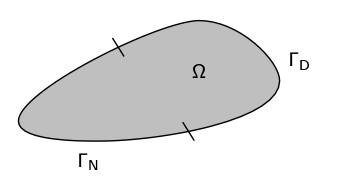
\includegraphics[width=0.8\linewidth]{images/tr3}
\end{Figure}
\end{multicols*}

% Restore the original parameters
\setlength{\columnseprule}{\oldcolumnseprule}

\rule{0.47\textwidth}{0.2pt}

\smallskip

\textbf{Weak Formulation.} Take a test function $v$ in a suitable functional space $V$, multiply ADR eq by $v$ and then integrate over $\Omega$:
\begin{equation*}
\int_\Omega \big[-\Div( \mu \nabla u )+\bv\cdot\nabla u+\sigma u\big] v=\int_\Omega fv
\end{equation*}

By parts we get
\begin{equation*}
\int_\Omega \mu \nabla u \cdot \nabla v-{\color{blue} \underbracket[0.5pt]{\int_{\partial \Omega} \mu \nabla u\cdot \nv\ v}_{\text{split}} } + \int_\Omega \bv\cdot \nabla u\ v+ \int_\Omega \sigma u v = \int_\Omega fv
\end{equation*}

Since we want $v$ behaves as $u$, we impose $v\big|_{\Gamma_D}=0$. Then the blue term becomes
\begin{equation*}
\int_{\partial \Omega} \mu \nabla u\cdot \nv\ v = \int_{\Gamma_D} \mu \nabla u\cdot \nv\ \cancel{v}+\int_{\Gamma_N} \underbracket[0.5pt]{\,\mu \nabla u\cdot \nv\,}_{=g}\ v
\end{equation*}

Finally, since $v$ is arbitrary, we obtain
\begin{equation*}
\underbracket[0.5pt]{\int_\Omega \mu \nabla u \cdot \nabla v+ \int_\Omega \bv\cdot \nabla u\ v+ \int_\Omega \sigma u v}_{\eqcolon a(u,v)} = \underbracket[0.5pt]{\int_\Omega fv + \int_{\Gamma_N} gv}_{\eqcolon F(v)}\qquad \forall\, v\in V
\end{equation*}

So the weak formulaton (WF) of problem \eqref{eqn:ADRproblem} is
\begin{equation*}
\boxed{
    \begin{gathered}
    \text{Find }u\in V=\left\{ v\in H^1(\Omega),\,v\big|_{\Gamma_D}=0 \right\}\eqcolon H^1_{\Gamma_D}(\Omega)\text{ s.t.} \\
    \int_\Omega \mu \nabla u \cdot \nabla v+ \int_\Omega \bv\cdot \nabla u\ v+ \int_\Omega \sigma u v = \int_\Omega fv + \int_{\Gamma_N} gv\qquad \forall\, v \in V
    \end{gathered}
}
\end{equation*}

In a more general framework, our abstract weak formulation is
\begin{equation*}
\boxed{\text{Find } u\in V\ :\ a(u,v)=F(v)\quad\forall\, v\in V} \tag{AWF}
\end{equation*}
where

% Save the current parameters
\let\oldcolumnseprule\relax
\newlength{\oldcolumnseprule}

\setlength{\oldcolumnseprule}{\columnseprule}

% Set new parameters for the new multicol environment
\setlength{\columnseprule}{0pt} % No separator rule

\begin{multicols*}{2}
% Your content here
\begin{itemize}
    \item $a:V\times V\to \RR$ bilinear form
    \item $F:V\to\RR$ linear form
\end{itemize}
\end{multicols*}

% Restore the original parameters
\setlength{\columnseprule}{\oldcolumnseprule}

\newcolumn

Now we need sufficient conditions for well-posedness.

\begin{theorem}[\bfseries Lax-Milgram Lemma] 
Assume that:
\begin{enumerate}[label=\textit{(\roman*)}]
\item $V$ Hilbert space with norm $\norm{\cdot}_V$ and inner product $(\cdot,\cdot)$
\item $F\in V'$ (linear and continuous/bdd functional over $V\!$), i.e. 
\begin{equation*}
\exists\,B>0 \qquad\text{s.t.}\qquad\abs{F(v)}\leq B\norm{v}_V\qquad\forall\,v\in V 
\end{equation*}

Note that $0<B\leq \norm{F}_{V'}\coloneq \displaystyle\sup_{\substack{v\in V \\ v\neq 0}} \frac{\abs{F(v)}}{\norm{v}_V} $ 

\item $a$ continuous, i.e. 
\begin{equation*}
\exists\,M>0 \qquad\text{s.t.}\qquad \abs{a(u,v)}\leq M \norm{u}_V\norm{v}_V\qquad \forall\,u,v\in V
\end{equation*}

\item $a$ coercive, i.e.
\begin{equation*}
\exists\,\alpha>0 \qquad\text{s.t.}\qquad a(v,v)\geq \alpha \norm{v}_V^2 \qquad\forall\,v \in V
\end{equation*}

\end{enumerate}
Then, $\exists\,!\ u$ solution of {\normalshape{(AWF)}}. 
\end{theorem}\vspace{-0.2cm}

As a corollary, from the following simple computation
\begin{gather}
\alpha \norm{u}_V^2 \overset{(iv)}{\leq} a(u,u) \overset{\text{AWF}}{=} F(u) \overset{(ii)}{\leq} \norm{F}_{V'} \norm{u}_V \nonumber \\
\Longrightarrow\quad \norm{u}_V \leq \frac{1}{\alpha}\, \norm{F}_{V'} \label{eqn:contData}
\end{gather}
we obtain a stability estimate / continuous dependence on data.

\smallskip

\emph{Rmk}: if $a(\cdot,\cdot)$ is additionally symmetric, then AWF is equivalent to the following variational problem:
\begin{equation*}
\begin{gathered}
\boxed{\text{Find }u\in V\ :\ u=\min_{v\in V} J(v)} \\
\text{where } J(v)\coloneq \frac{1}{2}\,a(v,v)-F(v) \qquad \forall\,v\in V
\end{gathered}
\end{equation*}

Questions:
\begin{itemize}
    \item How to prove assumptions of Lax-Milgram Lemma?

    $\qquad\qquad \to$ case by case, see below some examples

    \item What if the assumptions are not satisfied (in particular, coercivity)? 

    $\qquad\qquad \to$ see in the second part of the course
\end{itemize}

\rule{0.47\textwidth}{0.2pt}

\smallskip

Some useful tools you need when checking LM assumptions:
\begin{itemize}
    \item the space $H^1(\Omega)$ endowed with the energy norm
    \begin{equation*}
    \norm{v}_{H^1(\Omega)}^2\coloneq \norm{v}_{L^2(\Omega)}^2+\norm{\nabla v}_{L^2(\Omega)}^2 \qquad \forall\,v\in  H^1(\Omega)
    \end{equation*}

    and the scalar product
    \begin{equation*}
    (u,v)\coloneq (u,v)_{L^2(\Omega)}+(\nabla u,\nabla v)_{L^2(\Omega)}\qquad \forall\,u,v\in  H^1(\Omega)
    \end{equation*}

    is a Hilbert space

    \item the spaces $H^1_0(\Omega)$ and $H^1_{\Gamma_D}(\Omega)$ endowed with $\norm{\cdot}_{H^1(\Omega)}$ are Hilbert spaces because they are closed subspaces of $H^1(\Omega)$
\end{itemize}

Last but not least:

\begin{theorem}[\bfseries Poincaré Inequality]
Depending on the Sobolev space we'are considering, the following hold:

\begin{itemize}
    \item for the Poisson/diffusion problem
    \begin{equation}
    \label{eqn:PoincarePoisson}
    \exists\,C_\Omega>0\ :\ \norm{v}_{L^2(\Omega)}\leq C_\Omega \norm{\nabla v}_{L^2(\Omega)}\quad \forall\, v\in H^1_0(\Omega)
    \end{equation}
    $\leadsto$ on $H^1_0$ the norms $\norm{v}_{H^1(\Omega)}$ and $\norm{\nabla v}_{L^2(\Omega)}\eqcolon\norm{v}_{H^1_0(\Omega)}$ are equivalent.
    \item for the ADR problem (if meas$\,\left(\Gamma_D\right)>0$)
    \begin{equation}
    \label{eqn:PoincareADR}
    \exists\,C_\Omega>0\ :\ \norm{v}_{L^2(\Omega)}\leq C_\Omega \norm{\nabla v}_{L^2(\Omega)}\quad \forall\, v\in H^1_{\Gamma_D}(\Omega)
    \end{equation}
\end{itemize}

Therefore, wheter $V=H^1_0(\Omega)$ or $V=H^1_{\Gamma_D}(\Omega)$ there holds
\begin{gather}
\norm{v}_V^2=\norm{v}_{H^1}^2\coloneq \norm{v}_{L^2(\Omega)}^2+\norm{\nabla v}_{L^2(\Omega)}^2 \leq \left( 1+C_\Omega^2 \right)\norm{\nabla v}_{L^2(\Omega)}^2 \nonumber \\
\label{eqn:PoincareUsed}
\Longrightarrow \quad \norm{\nabla v}_{L^2(\Omega)}^2 \geq \frac{1}{1+C_\Omega^2}\,\norm{v}_V^2
\end{gather}

\end{theorem}\vspace{-0.2cm}

\begin{theorem}[\bfseries Trace Inequality]
For the ADR problem:
\begin{equation}
\label{eqn:traceADR}
\exists\,C_{\text{trace}}>0\ :\ \norm{v}_{L^2(\Gamma_N)}\leq C_{\text{trace}} \norm{v}_{V}\quad \forall\, v\in V\equiv H^1_{\Gamma_D}(\Omega)
\end{equation}
\end{theorem} \vspace{-0.2cm}

Checking LM assumptions on the Poisson problem ($\mu\in\RR^+$):
\begin{equation*}
\label{eqn:PoissonproblemStrong}
\textit{strong form}\quad \leadsto\quad
\left\{
\begin{array}{ll}
-\mu \Delta u=f &\text{in }\Omega \\
u=0 &\text{on }\partial\Omega 
\end{array}
\right.
\end{equation*}

\begin{equation*}
\textit{weak form}\quad \leadsto\quad
\boxed{
\begin{gathered}
\text{Find }u\in V\equiv H^1_0\text{ s.t.} \\
\int_\Omega \mu \nabla u\cdot\nabla v=\int_\Omega fv\qquad\forall \,v\in V
\end{gathered}}
\end{equation*}

\begin{enumerate}[label=\textit{(\roman*)}]
\item $V$ is Hilbert
\item $\forall\, v \in V$
\begin{equation*}
\abs{F(v)}=\abs{\int_\Omega fv}\overset{\text{cs}}{\leq} \norm{f}_{L^2(\Omega)} \norm{v}_{L^2(\Omega)} \leq \underbracket[0.5pt]{\norm{f}_{L^2(\Omega)}}_{=B} \norm{v}_{V} 
\end{equation*}
\item $\forall\, u,v \in V$
\begin{equation*}
\abs{a(u,v)}=\abs{\int_\Omega \mu \nabla u\cdot \nabla v}\overset{\text{cs}}{\leq}\mu \norm{\nabla u}_{L^2(\Omega)} \norm{\nabla v}_{L^2(\Omega)} \leq \mu \norm{u}_{V} \norm{v}_{V}
\end{equation*}
\item $\forall\, v \in V$
\begin{equation*}
a(v,v)=\int_\Omega\mu (\nabla v)^2=\mu\norm{\nabla v}^2_{L^2(\Omega)}\overset{\eqref{eqn:PoincareUsed}}{\geq} \underbracket[0.5pt]{\frac{\mu}{1+C_\Omega^2}}_{=\alpha}\,\norm{v}_V^2 
\end{equation*}
\item[$\Longrightarrow$] LM holds
\end{enumerate}

\smallskip

Checking LM assumptions on the ADR problem \eqref{eqn:ADRproblem} $\left( V\equiv H^1_{\Gamma_D} \right)$:
\begin{enumerate}[label=\textit{(\roman*)}]
\item $V$ is Hilbert
\item $\forall\, v \in V$
\begin{align*}
\abs{F(v)}&\leq\abs{\int_\Omega fv}+\abs{\int_{\Gamma_N} gv} \\
&\overset{\text{cs}}{\leq} \norm{f}_{L^2(\Omega)} \norm{v}_{L^2(\Omega)}+\norm{g}_{L^2(\Gamma_N)} \norm{v}_{L^2(\Gamma_N)} \\
& \overset{\eqref{eqn:traceADR}}{\leq} \underbracket[0.5pt]{\left( \norm{f}_{L^2(\Omega)}+C_{\textit{trace}} \norm{g}_{L^2(\Gamma_N)}  \right)}_{=B} \norm{v}_V
\end{align*}
\item $\forall\, u,v \in V$
\begin{align*}
\abs{a(u,v)}\leq&\abs{\int_\Omega \mu \nabla u\cdot \nabla v}+ \abs{\int_\Omega \bv\cdot \nabla u\ v}+\abs{\int_\Omega \sigma u v} \\
\overset{\text{cs}}{\leq}& \norm{\mu}_\infty \norm{\nabla u}_{L^2(\Omega)} \norm{\nabla v}_{L^2(\Omega)} + \\
&\norm{\bv}_\infty \norm{\nabla u}_{L^2(\Omega)} \norm{ v}_{L^2(\Omega)}+ \\
& \norm{\sigma}_\infty \norm{ u}_{L^2(\Omega)} \norm{ v}_{L^2(\Omega)} \\
\leq& \underbracket[0.5pt]{\left( \norm{\mu}_\infty+\norm{\bv}_\infty+\norm{\sigma}_\infty \right)}_{=M} \norm{u}_V \norm{v}_V
\end{align*}

\item $\forall\, v \in V$
\begin{gather*}
a(v,v)=\int_\Omega \mu(\nabla v)^2+{\color{teal} \underbracket[0.5pt]{\int_\Omega \bv\cdot\nabla v\ v}_{\text{by parts }\downarrow}}+\int_\Omega \sigma v^2= \\
\left\{ \int_\Omega \bv\cdot\nabla v\ v= \int_\Omega\bv\cdot \frac{1}{2}\,\nabla(v^2)\,{\color{teal}=\frac{1}{2} \int_{\Gamma_N} \bv\cdot\nv\ v^2 - \frac{1}{2} \int_\Omega \Div{(\bv)}\ v^2} \right\} \\
\geq \underbracket[0.5pt]{\min_{\xv\in\Omega} \mu(\xv)}_{\eqcolon \mu_0} \norm{\nabla v}_{L^2(\Omega)}^2+\int_\Omega \left( \sigma- \frac{1}{2}\,\Div{(\bv)} \right) v^2+ \frac{1}{2}\int_{\Gamma_N} \bv\cdot\nv\ v^2 
\end{gather*}

If we assume the following compatibility conditions
\begin{equation*}
\sigma- \frac{1}{2}\,\Div{(\bv)}\geq 0\ \text{ in }\Omega\qquad\qquad \bv\cdot \nv \geq 0\ \text{ on }\Gamma_N
\end{equation*}

then we'are able to prove coercivity:
\begin{equation*}
a(v,v)\geq \mu_0 \norm{\nabla v}_{L^2(\Omega)}^2 \overset{\eqref{eqn:PoincareUsed}}{\geq} \underbracket[0.5pt]{\frac{\mu_0}{1+C_\Omega^2}}_{=\alpha}\,\norm{v}_V^2 
\end{equation*}

\item[$\Longrightarrow$] LM holds BUT under the above-mentioned conditions
\end{enumerate}

\rule{0.47\textwidth}{0.2pt}

\smallskip

\textbf{Galerkin Approximation.} If we build $V_h\subseteq V$ (conforming setting) with $\text{dim }V_h=N_h<\infty$, then we can project the AWF on the finite dimensional space:
\begin{equation*}
\boxed{\text{Find } u_h\in V_h\ :\ a(u_h,v_h)=F(v_h)\quad\forall\, v_h\in V_h}\tag{G}
\end{equation*}

\newcolumn

Analysis of G:
\begin{itemize}
\item \emph{well-posedness} follows from LM (being $V_h$ a closed subspace of $V$)
\item \emph{stability} is the continuous dependence from data \eqref{eqn:contData}
\begin{equation*}
\norm{u_h}_V\leq \frac{1}{\alpha}\,\norm{F}_{V'} 
\end{equation*}
also known as uniform bound wrt $h$

\item \emph{consistency} $\equiv$ Galerkin orthogonality:
\begin{equation*}
a(u-u_h,v_h)=0\qquad\forall\, v_h\in V_h \tag{GO}
\end{equation*}

\begin{Figure}
    \centering
    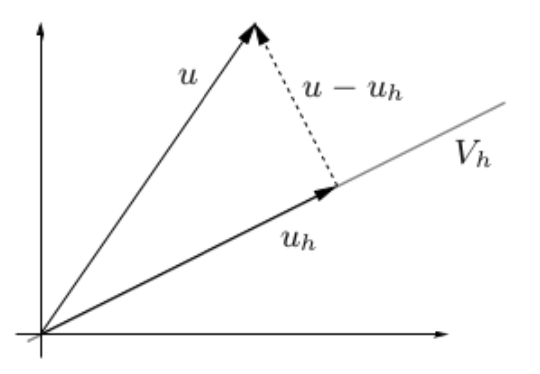
\includegraphics[width=0.4\linewidth]{images/GO}
\end{Figure}

\begin{proof}
Since AWF holds $\forall\,v\in V$, it holds $\forall\,v_h\in V_h\subseteq V$ too. Therefore, we subtract
\begin{equation*}
\begin{array}{cll}
 & a(u,v_h)=F(v_h) & \forall\,v_h\in V_h \\
- & & \\
 & \underbracket[0pt]{a(u_h,v_h)=F(v_h)}_{\quad} & \forall\,v_h\in V_h \\
\hline
 & \overbracket[0pt]{a(u-u_h,v_h)=0}^{\quad} & \forall\,v_h\in V_h
\end{array} 
\end{equation*}
\end{proof}

\item \emph{convergence} $\equiv$ space saturation + Céa Lemma
\begin{gather*}
\lim_{h\to 0}\inf_{v_h\in V_h}\norm{v-v_h}_V=0\quad\forall\, v\in V \tag{SP} \\
\norm{u-u_h}_V\leq \frac{M}{\alpha}\,\inf_{v_h\in V_h}\norm{u-v_h}_V \tag{CL}
\end{gather*}

\emph{Rmk}: because in general $\nicefrac{M}{\alpha}\neq 1$ we have \emph{quasi-optimality}.

\begin{proof}
We have
\begin{align*}
\alpha\norm{u-u_h}_V^2&\overset{(iv)}{\leq} a(u-u_h,u-u_h) \\
&\,\,=a(u-u_h,u\,{\color{green}-v_h+v_h}-u_h) \\
&\,\,=a(u-u_h,u-v_h)+\underbracket[0.5pt]{a(u-u_h,\underbracket[0.5pt]{v_h-u_h}_{\eqcolon w_h})}_{=0\text{ by GO}} \\
&\overset{(iii)}{\leq} M \norm{u-u_h}_V \norm{u-v_h}_V\quad \forall\,v_h\in V_h \\
\Longrightarrow\quad \underbracket[0.5pt]{ \norm{u-u_h}_V }_{\text{error}}&\leq \frac{M}{\alpha}\,\norm{u-v_h}_V\quad\forall\,v_h\in V_h \\
\overset{\text{inf }}{\Longrightarrow}\quad \norm{u-u_h}_V &\leq \frac{M}{\alpha}\,\inf_{v_h\in V_h}\norm{u-v_h}_V \xrightarrow{h\to 0} 0
\end{align*}
by the space saturation assumption.
\end{proof}
\end{itemize}

Last but not least: 
\begin{theorem}
Problem {\normalshape{(G)}} is equivalent to the following linear system of equations:
\begin{equation*}
\boxed{\text{\normalfont Find } \uv\in\RR^{N_h}\ :\ A\uv=\Fv}\tag{LS}
\end{equation*}
where $A\in\RR^{N_h\times N_h},\ \Fv\in\RR^{N_h}$.    
\end{theorem}\vspace{-0.5cm}

\begin{proof}
$V_h$ has finite dimension, meaning that
\begin{equation*}
V_h=\text{span }\left\{ \phi_1,\dots,\phi_{N_h} \right\}
\end{equation*}

Then $u_h\in V_h$ is written as
\begin{equation*}
u_h=\sum_{j=1}^{N_h} u_j\phi_j
\end{equation*}

We put it in G to obtain
\begin{align*}
\text{Find } \left\{ u_j \right\}_{j=1}^{N_h}\text{ s.t. } & a \left( \sum_{j=1}^{N_h} u_j\phi_j,v_h  \right)=F(v_h) && \forall\,v_h\in V_h \\
& a \left( \sum_{j=1}^{N_h} u_j\phi_j,\phi_i  \right)=F(\phi_i) && \forall\,i=1,\dots,N_h \\
& \sum_{j=1}^{N_h} u_j\, \underbracket[0.5pt]{a(\phi_j,\phi_i)}_{\eqcolon A_{ij}}=\underbracket[0.5pt]{F(\phi_i)}_{\eqcolon F_{i}} && \forall\,i=1,\dots,N_h
\end{align*}

and this is exactly LS.
\end{proof}

Moral of the story: $V_h$ must be chosen to ensure the density property (SP) and the computation of the integrals $A_{ij}$ and $F_i$.

\newpage

\textbf{The Finite Element Method.} We consider a domain $\Omega$ with polygonal shape (we do not take into account error due to the approximation of a non-polygonal domain with a FE grid). 
\begin{Figure}
    \centering
    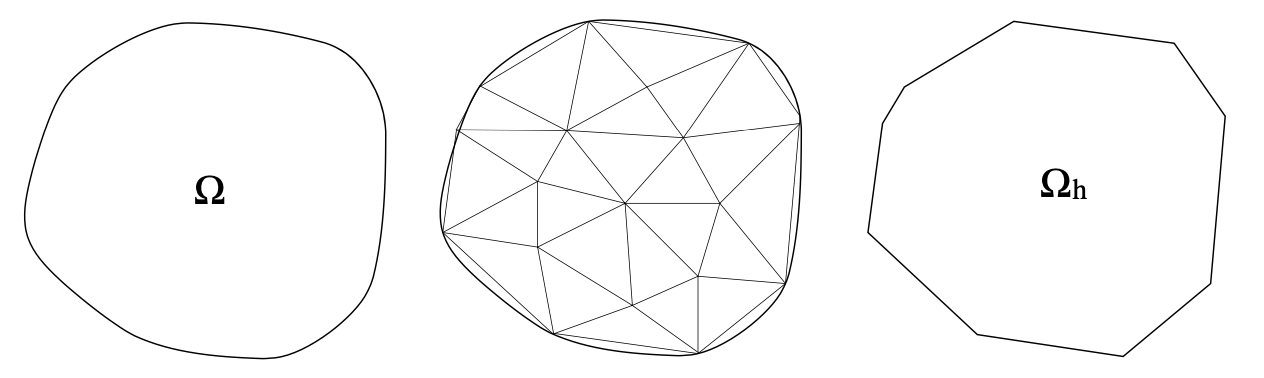
\includegraphics[width=\linewidth]{images/poly_shapes}
\end{Figure}

Therefore, our first hypothesis is that the approximation $\Omega_h$ of the domain $\Omega$ is such that
\begin{equation*}
\lim_{h\to 0} \emph{meas}\,(\Omega-\Omega_h)=0
\end{equation*}

\rule{0.47\textwidth}{0.2pt}

\smallskip

Then we define as \textbf{mesh} a finite cover of $K$ non-overlapping triangles, also called \emph{triangulation} (in broad sense) of $\Omega$ (of $\Omega_h$ actually, for the previous hypothesis): 
\begin{equation*}
\Tc_h=\bigcup K
\end{equation*}

To make it clearer: in 1D, intervals; in 2D, triangles but we'll see also quadrilaterals; in 3D, tetrahedra but we'll see also hexahedra.

Since the triangles are non-overlapping there holds
\begin{equation*}
\overset{\circ}{K_i}\cap \overset{\circ}{K_j} = \emptyset\qquad \forall\,K_i,K_j\in\Tc_h\,:\,K_i\neq K_j
\end{equation*}

where $\overset{\circ}{K}=K\setminus\partial K$ is the interior of $K$.

In addiction, we suppose that 
\begin{equation*}
\begin{gathered}
\text{if }F=K_i\cap K_j\neq \emptyset \qquad \text{with }K_i,K_j\in\Tc_h\,:\,K_i\neq K_j \\
\text{then }F\text{ is either a whole edge (face) or a vertex of the grid}
\end{gathered}
\end{equation*}

In this way we are avoiding hanging nodes, and the mesh is said to be \emph{conforming}.
\begin{Figure}
    \centering
    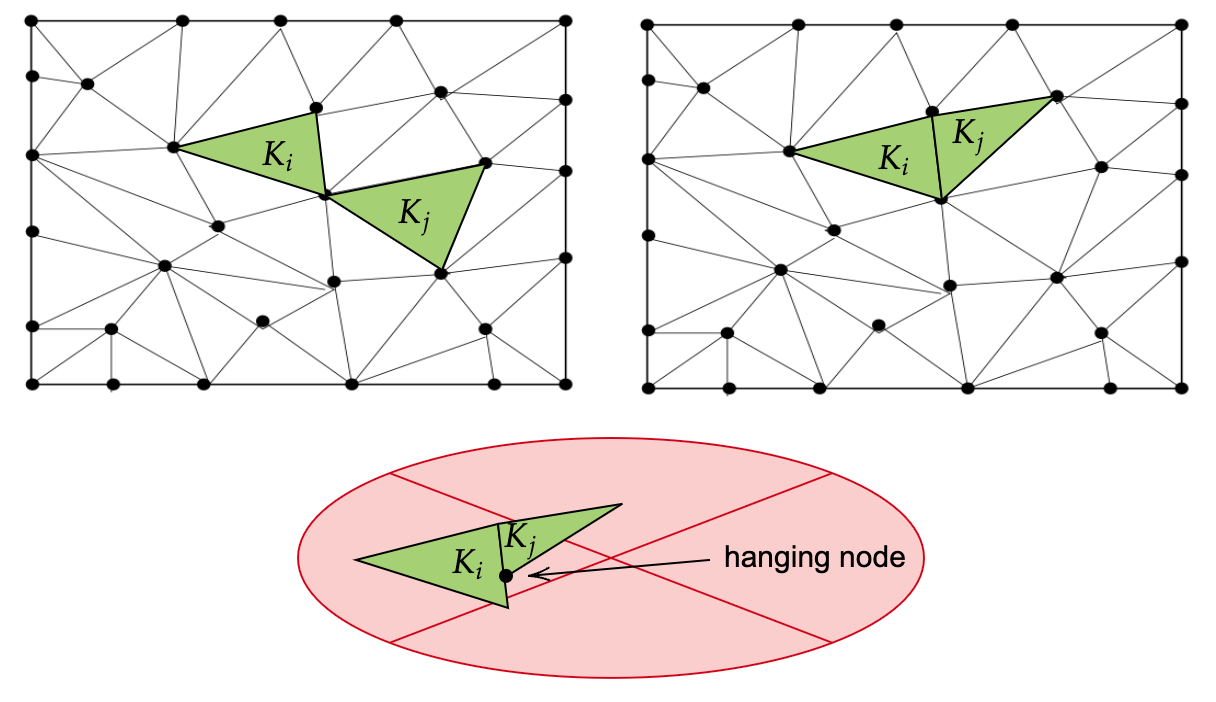
\includegraphics[width=\linewidth]{images/hanging}
\end{Figure}

\rule{0.47\textwidth}{0.2pt}

\smallskip

We then set
\begin{equation*}
h_K=\text{diam}\,(K)\qquad\forall\,K\in\Tc_h
\end{equation*}
and
\begin{equation*}
h=\max_{K\in\Tc_h} h_K
\end{equation*}

which represents the spacing of the grid.

\rule{0.47\textwidth}{0.2pt}

\smallskip

In dimension $d=1,2,3,\dots$, we denote by $\PP^r$ the space of polynomials of total degree $\leq r$:
\begin{equation*}
\begin{aligned}
&d=1,\ \PP^r:\qquad && p(x)=\sum_{k=0}^r a_k\, x^k \\
&d=2,\ \PP^r:\qquad && p(x,y)=\sum_{\substack{k=0,\dots,r \\
m=0,\dots,r \\
k+m\leq r} }  a_{km}\, x^k y^m \\
&d=3,\ \PP^r:\qquad && p(x_1,x_2,x_3)=\sum_{\substack{k=0,\dots,r \\
m=0,\dots,r \\
n=0,\dots,r \\
k+m+n\leq r} }  a_{kmn}\, x_1^k \, x_2^m\, x_3^n \\
\end{aligned}
\end{equation*}

Instead, $\QQ^r$ is the space of polynomials of degree in each variables $\leq r$:
\begin{equation*}
d=3,\ \QQ^r:\qquad p(x_1,x_2,x_3)=\sum_{\substack{k=0,\dots,r \\
m=0,\dots,r \\
n=0,\dots,r} }  a_{kmn}\, x_1^k \, x_2^m\, x_3^n
\end{equation*}

The dimension of the spaces $\PP^r$ is obtained via the following formula:
\begin{equation*}
\text{dim}\,\big(\PP^r\big)=\frac{(r+d)\,!}{r\,!\ d\,!} 
\end{equation*}

For example, in the two-dimensional case, since $\text{dim}\left( \PP^r \right)=\nicefrac{(r+1)(r+2)}{2}$, on every triangle of the grid $\Tc_h$ a generic function $v_h$ is well-defined whenever its value at 3, 6, 10 nodes is known for $\PP^1$, $\PP^2$, $\PP^3$:
\begin{Figure}
    \centering
    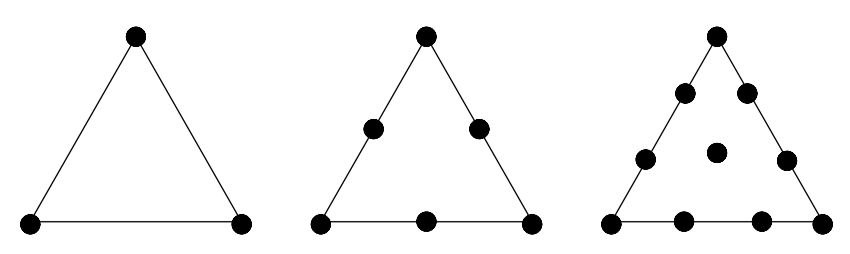
\includegraphics[width=0.7\linewidth]{images/tr1}
\end{Figure}

Instead, for tetrahedron we have:
\begin{Figure}
    \centering
    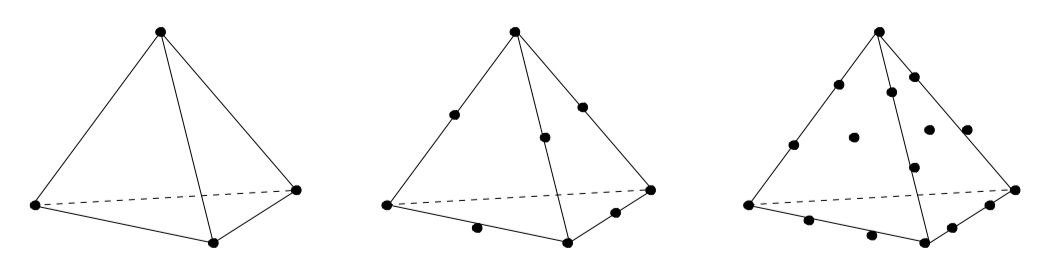
\includegraphics[width=0.8\linewidth]{images/tr2}
\end{Figure}

\rule{0.47\textwidth}{0.2pt}

Finally, we can introduce our finite element space ($r\geq 1$):
\begin{equation*}
V_h\coloneq \left\{ v_h\in\Cc^0(\overline{\Omega})\,:\,v_h\big|_{K}\in\PP^r(K)\ \ \forall\,K\in\Tc_h,\ v_h\big|_{\Gamma_D}=0  \right\}
\end{equation*}

We notice that:
\begin{itemize}
\item $v_h\in\Cc^0(\overline{\Omega})$, but how are we going to impose continuity over the triangles?

Let's answer in the case $d=2$, $r=1$. If you restrict a linear polynomial to an edge, it is still a linear polynomial. Therefore, to impose the continuity between two triangles of our mesh, it is sufficient to impose that the values at the two vertices are equal. This is because $\text{dim}\,(\PP^r)=r+1=2$. For higher degrees or dimensions, the reasoning is the same: just look at the figure of the triangles above!

Instead, if the mesh is made up with quads, the continuity enforcement is not possible in $\PP^r$. At least, you need to be in $\QQ^r$.

\item $v_h\big|_{\Gamma_D}=0$, that's why the Dirichlet boundary condition is called \emph{essential}: you have to impose it on the space!
\end{itemize}

Is this choice of $V_h$ suitable for the space saturation assumption and the computation of the integrals?

\rule{0.47\textwidth}{0.2pt}

\textbf{Error Analysis.} Recall the Céa Lemma (CL):
\begin{equation*}
\begin{aligned}
\norm{u-u_h}_V&=\norm{u-u_h}_{H^1(\Omega)} \\
&\leq \frac{M}{\alpha} \inf_{v_h\in V_h} \norm{u-v_h}_{H^1(\Omega)} \\
&\leq \frac{M}{\alpha}\, \norm{u-\overline{v_h}\,}_{H^1(\Omega)}
\end{aligned}
\end{equation*}

for a partical choice of $\overline{v_h}\in V_h$. Let $\overline{v_h}=\prod_h^r u$ the finite element interpolant of $u$. Then we have:
\begin{equation}
\label{eq:interbds}
\norm{u-u_h}_V\leq \frac{M}{\alpha}\, \underbracket[0.5pt]{\norm{u-\textstyle\prod_h^r u}_{H^1(\Omega)}}_{\substack{\text{interpolation}\\\text{problem}}}
\end{equation}

\begin{theorem}[\bfseries Interpolation error bounds]
For any $v\in H^{r+1}(\Omega)$, $r\geq 1$, $\exists\,C$ such that
\begin{equation*}
\abs{v-\textstyle\prod_h^r v}_{H^m(\Omega)}\leq C_{m,r} \left( \sum_{K\in\Tc_h} h_K^{2(r+1-m)}\abs{v}^2_{H^{r+1}(\Omega)} \right)^{1/2}\quad m=0,1
\end{equation*}

Recalling that $H^0(\Omega)\equiv L^2(\Omega)$ and that $\abs{\cdot}_{H^m(\Omega)}$ is the seminorm, which is defined as
\begin{equation*}
\abs{v}_{H^m(\Omega)}\coloneq \norm{v^{(m)}}_{L^2(\Omega)}\qquad \forall\, m\geq 0
\end{equation*}

(where $v^{(0)}\equiv v$), we can state that provided v \emph{regular enough} (i.e. to have the seminorm bounded) there hold:
\begin{align}
\label{eq:bdsl2}
\norm{v-\textstyle\prod_h^r v}_{L^2(\Omega)}\leq C h^{r+1} \abs{v}_{H^{r+1}(\Omega)}
\\
\label{eq:bdsh1}
\abs{v-\textstyle\prod_h^r v}_{H^1(\Omega)}\leq C h^r \abs{v}_{H^{r+1}(\Omega)}
\end{align}
\end{theorem}\vspace{-0.3cm}

Hence, we can finally bound the full $V$-norm, since its definition is
\begin{equation*}
\norm{u}_{H^1(\Omega)}\coloneq \left( \norm{u}_{L^2(\Omega)}^2+ \abs{u}_{H^1(\Omega)}^2 \right)^{1/2}
\end{equation*}

Indeed from \eqref{eq:interbds}, using \eqref{eq:bdsl2} and \eqref{eq:bdsh1}, we get
\begin{equation*}
\norm{u-u_h}_V\leq \frac{M}{\alpha} \,\norm{u-\textstyle\prod_h^r u}_{H^1(\Omega)} \overset{\circledast}{\leq} C\,\frac{M}{\alpha}\,h^{r}\abs{u}_{H^{r+1}(\Omega)} 
\end{equation*}

which, moreover, guarantees (SP).

\smallskip

$\circledast$ if you want to be explicit when using \eqref{eq:bdsl2} and \eqref{eq:bdsh1} you have to carefully deal with the two components of the $H^1$-norm.

\newpage

Let's sum it up in a theorem:
\begin{theorem}[\bfseries $\bm {H^1(\Omega)}$ error bounds]
Let $u\in V$ be the solution of {\normalshape{(AWF)}} and suppose $u\in H^{r+1}(\Omega)$, $r\geq 1$. Let $u_h$ be the finite element solution of {\normalshape{(G)}}. Then $\exists\,C=C_r$ such that
\begin{equation}
\label{eq:finalH1bds}
\norm{u-u_h}_V\lesssim h^r\abs{u}_{H^{r+1}(\Omega)}
\end{equation} 
\end{theorem}\vspace{-0.2cm}

It follows from the latter theorem that, in order to increase the accuracy, two different strategies can be followed: reducing $h$, i.e. refining the grid, or increasing $r$, that is using finite elements of higher degree. 

\smallskip

However, increasing $r$ makes sense only if the solution $u$ is regular enough: as a matter of fact, from \eqref{eq:finalH1bds} we immediately infer that, if $u \in V \cap H^{p+1}(\Omega)$, the maximum value of $r$ that it makes sense to take is $r = p$. Values higher than $p$ do not ensure a better rate of convergence: therefore if the solution is not very regular it is not convenient to use finite elements of high degree, as the greater computational cost is not compensated by an improvement of the convergence. 

\smallskip

An interesting case is when the solution only has the minimum regularity $(p = 0)$. From the relations (CL) and (SP) we obtain that there is anyhow convergence, but estimate \eqref{eq:finalH1bds} is no longer valid. It is then impossible to say how the norm $V$ of the error tends to zero when $h$ decreases. We summarize these situations in the following table:

\begin{Figure}
    \centering
    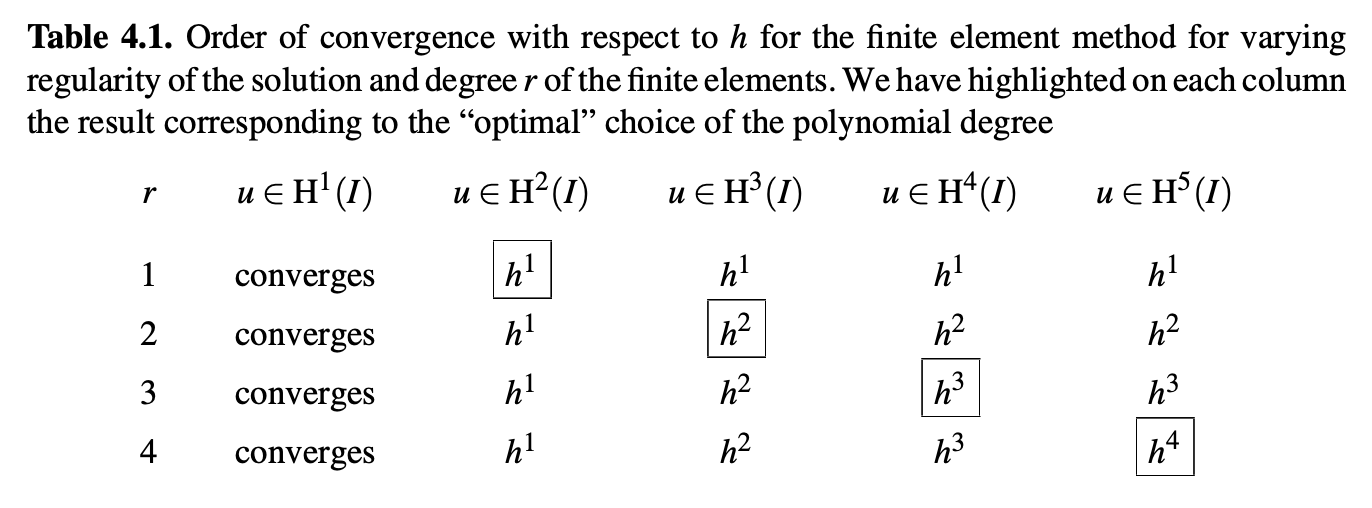
\includegraphics[width=\linewidth]{images/Q1}
\end{Figure}

In general, we can state that: if $u \in H^{p+1}(\Omega)$, for a given $p > 0$, then there exists a constant $C$ independent of $u$ and $h$, such that
\begin{equation*}
\norm{u-u_h}_{H^1(\Omega)} \leq C h^s |u|_{H^{s+1}(\Omega)} \qquad s = \min\{r,p\}
\end{equation*}

The last part is about the:
\begin{theorem}[\bfseries $\bm {L^2(\Omega)}$ error bounds]
Let $u\in V$ be the solution of {\normalshape{(AWF)}} and suppose $u\in H^{r+1}(\Omega)$, $r\geq 1$. Let $u_h$ be the finite element solution of {\normalshape{(G)}}. Then $\exists\,C=C_r$ such that
\begin{equation}
\label{eq:finalL2bds}
\norm{u-u_h}_V\lesssim h^{r+1}\abs{u}_{H^{r+1}(\Omega)}
\end{equation}
\end{theorem}\vspace{-0.2cm}

In simple words, in $L^2(\Omega)$ \emph{you gain one order}.

\begin{proof}
Consider a bilinear form $a:V\times V\to\RR$. The adjoint form $a^*$ is defined as:
\begin{equation*}
a^*:V\times V\to\RR \qquad a^*(v,w)\coloneq a(w,v)\quad\forall\,v,w\in V
\end{equation*}

Assume $a$ symmetric (then $a^*\equiv a$) and consider the following adjoint problem:
\begin{equation}
\label{eq:adjointPRB}
\begin{gathered}
\text{Given }g\in L^2(\Omega), \text{ find }\phi\in V\text{ such that}\\
a^*(\phi,v)=\int_\Omega g\,v\qquad\forall\,v\in V
\end{gathered}
\end{equation}

Assume there holds LM, then $\exists\,!\  \phi$ weak solution to \eqref{eq:adjointPRB}. Moreover, by elliptic regularity, we have that $\phi\in H^2(\Omega)\cap V$ and $\exists\, C>0$ such that
\begin{equation}
\label{eq:adjEstim}
\norm{\phi(g)}_{H^2(\Omega)}\leq C \norm{g}_{L^2(\Omega)}
\end{equation}

Take now $g\equiv u-u_h$. Clearly $g\in L^2(\Omega)$ and
\begin{equation*}
\begin{aligned}
\norm{u-u_h}_{L^2(\Omega)}^{\cancel{2}} & = (u-u_h,u-u_h)_{L^2(\Omega)} \\
&\overset{\eqref{eq:adjointPRB}}{=} a^* (\phi,u-u_h) \\
&\overset{a\text{ sym}}{=}a(u-u_h,\phi) \\
&\overset{\text{GO}}{=}a(u-u_h,\phi-\phi_h) \qquad (\text{for }\phi_h\in V_h) \\
&\overset{a\text{ cont}}{\leq} M \norm{u-u_h}_{H^1(\Omega)}\norm{\phi-\phi_h}_{H^1(\Omega)} \\
&\overset{\text{choose }\phi_h}{\leq} M \norm{u-u_h}_{H^1(\Omega)}\norm{\phi-\textstyle\prod_h^1\phi}_{H^1(\Omega)} \\
&\overset{\eqref{eq:finalH1bds}}{\leq} MC_1 \norm{u-u_h}_{H^1(\Omega)} h\abs{\phi}_{H^2(\Omega)} \\
&\overset{\eqref{eq:adjEstim}}{\leq} MC_2\, h \norm{u-u_h}_{H^1(\Omega)} \norm{u-u_h}_{L^2(\Omega)} \\
&\overset{\eqref{eq:finalH1bds}}{\leq} MC_3\, h\, h^r\abs{u}_{H^{r+1}(\Omega)} \cancel{\norm{u-u_h}_{L^2(\Omega)}} \\
&\lesssim h^{r+1} \abs{u}_{H^{r+1}(\Omega)} 
\end{aligned}
\end{equation*}
\end{proof}

\rule{0.47\textwidth}{0.2pt}\smallskip

\textbf{Computation of the integrals.} See Tablet.

\bigskip

\rule{0.47\textwidth}{0.2pt}\smallskip

\textbf{Conditioning of the stiffness matrix.} We have seen that the stiffness matrix $A = \left[ a(\varphi_j, \varphi_i) \right]$ associated to the Galerkin problem and therefore, in particular, to the finite element method, is positive definite; moreover $A$ is symmetric if the bilinear form $a(\cdot, \cdot)$ is symmetric.

\smallskip

For a symmetric and positive definite matrix, its condition number with respect to the norm $\|\cdot\|_2$ is given by
\begin{equation}
\label{eq:tocond}
K_2(A) = \frac{\lambda_{\text{max}}(A)}{\lambda_{\text{min}}(A)}
\end{equation}
$\lambda_{\text{max}}(A)$ and $\lambda_{\text{min}}(A)$ being the maximum and minimum eigenvalues, respectively, of $A$. It can be proved that, both in the one-dimensional and the multi-dimensional case, the following relation holds for the stiffness matrix:
\begin{equation*}
K_2(A) = \Oc \big(h^{-2}\big)
\end{equation*}

When the grid-size $h$ decreases, the condition number of the stiffness matrix increases, and therefore \textbf{the associated system becomes more and more ill-conditioned}. In particular, if the datum $\fv$ of the linear system $A\uv=\fv$ is subject to a perturbation $\delta \fv$ (i.e. it is affected by error), the latter in turn affects the solution with a perturbation $\delta \uv$; then it can be proved that, if there are no perturbations on the matrix $A$,
\begin{equation*}
\frac{|\delta \uv|}{|\uv|} \leq K_2(A) \frac{|\delta \fv|}{|\fv|}
\end{equation*}

It is evident that \textbf{the higher the conditioning number is, the more the solution is affected by the perturbation on the data.}

\smallskip

As a further example we can study how conditioning affects the solution method. Consider, for instance, solving the linear system using the \textbf{conjugate gradient method}. Then a sequence $\mathbf{u}^{(k)}$ of approximate solutions is iteratively constructed, converging to the exact solution $\mathbf{u}$. In particular, we have
\begin{equation*}
\norm{\mathbf{u}^{(k)} - \mathbf{u}}_A \leq 2 \left( \frac{\sqrt{K_2(A)} - 1}{\sqrt{K_2(A)} + 1} \right)^k \norm{\mathbf{u}^{(0)} - \mathbf{u}}_A
\end{equation*}
having denoted by $\|\mathbf{v}\|_A = \sqrt{\mathbf{v}^T A \mathbf{v}}$ the so-called “A-norm” of a generic vector $\mathbf{v} \in \mathbb{R}^{N_h}$. If we define
\begin{equation*}
\rho = \frac{\sqrt{K_2(A)} - 1}{\sqrt{K_2(A)} + 1}
\end{equation*}
such quantity gives an idea of the convergence rate of the method: the closer $\rho$ is to 0, the faster the method converges, whilst the closer $\rho$ is to 1, the slower the convergence. Indeed, following \eqref{eq:tocond}, the more accurate one wants to be, by decreasing $h$, the more ill-conditioned the system will be, and therefore the more \emph{problematic} its solution will turn out to be.

\smallskip

This calls for the system to be \textbf{preconditioned}, i.e. it is necessary to find an invertible matrix $P$, called \textit{preconditioner}, such that
\begin{equation*}
K_2\big(P^{-1} A\big) \ll K_2(A)
\end{equation*}

and then apply the iterative method to the system preconditioned with $P$.

\smallskip

\emph{Remark:} how many iterations to reduce the relative error by a factor 10 with the gradient method?
\begin{equation*}
\rho^k<10^{-1}\quad \Longleftrightarrow\quad k>\frac{\log(10)}{\log(\rho)} 
\end{equation*}

\rule{0.47\textwidth}{0.2pt}












%!TEX root = ../main.tex


%!TEX root = ../main.tex

% =================================================

% \section{Discountinuous Galerkin Methods}

% =================================================
%!TEX root = ../main.tex

\end{multicols*}

\end{document}